\documentclass[10pt,pdf,hyperref={unicode}]{beamer}

\usepackage{graphicx}
\graphicspath{{./figs/}}

\mode<presentation> {
	\usetheme{Warsaw}
%	\usetheme{chpc}
	  
	\setbeamercovered{transparent}
  % or whatever (possibly just delete it)
}

\usepackage[english]{babel}
%\usepackage[utf8x]{inputenc}

%\usepackage{amsmath}
\usepackage{bm}
\usepackage{tikz}
\usepackage{pgfplots}

\title[] % (optional, use only with long paper titles)
{Multiscale Model Reduction \\for Neutron Diffusion Equation}

%\subtitle
%{Include Only If Paper Has a Subtitle}

\author[] % (optional, use only with lots of authors)
{Aleksandr Avvakumov \inst{1} \and Denis Spiridonov \inst{2} \\ 
\and \underline{Aleksandr Vasilev \inst{2}}}
% - Give the names in the same order as the appear in the paper.
% - Use the \inst{?} command only if the authors have different
%   affiliation.

\institute[Universities of Somewhere and Elsewhere] % (optional, but mostly needed)
{
\inst{1} National Research Center \textquotedblleft Kurchatov Institute\grqq, Moscow, Russia
\\
\vspace{1mm}
\inst{2} North-Eastern Federal University, Yakutsk, Russia
}

% - Use the \inst command only if there are several affiliations.
% - Keep it simple, no one is interested in your street address.

\date[September 9-12, 2020] % (optional, should be abbreviation of conference name)
{4th MHPCMP, September 9-12, 2020 Sochi}
% - Either use conference name or its abbreviation.
% - Not really informative to the audience, more for people (including
%   yourself) who are reading the slides online

\subject{Theoretical Computer Science}
% This is only inserted into the PDF information catalog. Can be left
% out. 

% ����� � ���������
\graphicspath{{./figs/}}
\newcommand{\grad}{\mathop{\rm grad}\nolimits}
\renewcommand{\div}{\mathop{\rm div}\nolimits}
\newcommand{\const}{\mathop{\rm const}\nolimits}

\begin{document}

\begin{frame}
  \titlepage
\end{frame}

%{
%  \begin{frame}<beamer>
%    \tableofcontents
%  \end{frame}
%}

\section{Introduction}
\begin{frame}{Introduction}
\end{frame}

\section{Problem statement}
\subsection{Diffusion approximation}
\begin{frame}{Problem statement}
	We consider a bounded 2D domain  $\Omega$ ($\bm x = \{x_1, x_2\} \in \Omega$) with a convex boundary $\partial \Omega$. 
	The one-group transport equation in the diffusion approximation with one-group delayed neutron source can be written as follows
	\begin{equation}\label{1}
		\begin{split}
			\frac{1}{v} \frac{\partial \phi}{\partial t} - \nabla \cdot D \nabla \phi + \Sigma_r \phi &= \frac{1 - \beta}{K_{eff}} \nu \Sigma_f \phi + \lambda c, \\
			\frac{\partial c}{\partial t} + \lambda c &= \frac{\beta}{K_{eff}} \nu \Sigma_f \phi.
		\end{split}
	\end{equation}
	Here $\phi(\bm x,t)$ is the neutron flux  at point $\bm x$ and time $t$,
	$v$ is the effective neutron velocity,
	$D(\bm x)$ is the diffusion coefficient, 
	$\Sigma_r(\bm x,t)$ is the removal cross-section,
	$\Sigma_f(\bm x,t)$ is the fission cross-section,
	$\beta$ is the effective fraction of delayed neutrons, 
	$\lambda$ is the decay constant of the delayed neutron source.
\end{frame}

\subsection{Boundary and initial conditons}
\begin{frame}{Boundary and initial conditons}
	Let's determine the boundary and initial conditions for Equation (\ref{1}).
	The albedo-type conditions are set at the boundary  $\partial \Omega$:
	\begin{equation}\label{2}
		D\frac{\partial \phi}{\partial n} + \gamma \phi = 0,
	\end{equation} 
	where $n$ is an outer normal to the boundary $\partial \Omega$, $\gamma$ is the albedo constant.
	Let's propose that at the initial time t = 0, the reactor is in steady-state critical condition
	\begin{equation}\label{3}
		\phi(\bm x,0) = \phi^0(\bm x).
	\end{equation} 
\end{frame}

\subsection{Discretization}
\begin{frame}{Time approximation}
	To solve the problem within the domain $\Omega$, we approximate the system of equations (\ref1)-(\ref{3}) using the finite element method.
	We discretize the time derivatives using finite-difference scheme, and then bring each stationary problem to a variational formulation. 
	For approximation in time, we use a fully implicit scheme with time step $\tau$. 
\end{frame}

\begin{frame}{Varitional formulation}
	To specify the variational formulation, we multiply equations by the test function $q$ and integrate over the domain $\Omega$. 
	Using the integration by parts, we obtain the following variational formulation: let's find $\phi^{n+1} \in V$ such that
	\begin{equation} \label{4}
	\begin{split}
		\int_\Omega \frac{1}{v} \frac{\phi^{n+1}}{\tau} q d\bm x +
		\int_\Omega D^{n+1} \nabla\phi^{n+1} \cdot \nabla q d\bm x &+ 
		\int_\Omega \Sigma_r^{n+1} \phi^{n+1} q d\bm x - \\
		\int_\Omega \frac{1+\lambda\tau-\beta}{K_{eff}(1+\lambda\tau)} \nu \Sigma_f^{n+1} \phi^{n+1} q d\bm x &+
		\int_{\partial \Omega} \gamma \phi^{n+1} q d\bm s = \\
		\int_\Omega \frac{1}{v} \frac{\phi^{n}}{\tau} q d\bm x +
		\int_\Omega \frac{\lambda c^n}{1+\lambda\tau} q d\bm x &, \quad \forall q \in V,
	\end{split}
	\end{equation}
	where $V=H^1(\Omega)$ is the Sobolev space consisting of scalar functions $\upsilon$ such that $\upsilon^2$ and $|\nabla \upsilon^2|$ have a finite integral in $\Omega$.
\end{frame}

\begin{frame}{Discrete problem}
	Further, it's necessary to pass from the continuous variational problem (\ref{4}) to the discrete problem. 
	We introduce finite-dimensional space of finite elements $V_h \subset V$ and formulate a discrete variational problem. 
	We use standard linear basis functions as basis functions to solve the problem on the fine grid.
	\\
	\begin{center}
		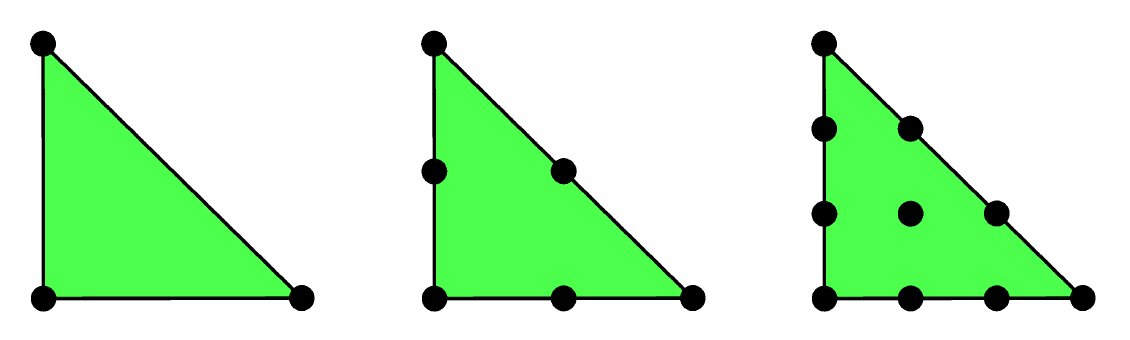
\includegraphics[width=0.5\linewidth] {triangle.png}
	\end{center}
\end{frame}


\section{Multiscale method}
\subsection{Algorithm}
\begin{frame}{Time step selection algorithm}
\begin{enumerate}
\item 
Predictable time step: $\widetilde{\tau}^{n+1} = \gamma \tau^n$ (eg $\gamma=1.25$)
\vspace{2mm}

\item Predictive solution $\widetilde{y}^{n+1}$: an explicit scheme, $\widetilde{t}^{n+1} = t^n + \widetilde{\tau}^{n+1}$
\vspace{2mm}

\item Estimation of approximation error: by found $\widetilde{y}^{n+1}$ from an implicit scheme
\vspace{2mm}

\item Step selection $\tau^{n+1}$: $\ \|\psi^{n+1}\| \approx \delta$
\vspace{2mm}

\item Solution on a new time layer $y^{n+1}$: an implicit scheme, $t^{n+1}=t^n + \tau^{n+1}$
\end{enumerate}
\end{frame}

\subsection{Neutron diffusion equation}
\begin{frame}{Neutron diffusion equation}
One group diffusion approximation with one group delayed neutron sources
\[
\begin{split}
 \frac{1}{v} \frac{\partial \phi}{\partial t} -  \nabla \cdot D \nabla \phi + \Sigma_{a} \phi &=   \ (1-\beta) \nu \Sigma_{f} \phi + \lambda c, \\
\frac{\partial c}{\partial t} + \lambda c &= \beta \nu \Sigma_{f} \phi.
\end{split}
\]

%\visible<2>{
Boundary condition
\[
 D\frac{\partial \phi}{\partial n} + \gamma_a \phi = 0.
\]

Initial conditions
\[
 \phi(0) = \phi^0,  \,
 c(0) = c^0.
\]
%}
\end{frame}

\subsection{Calculated formulas}
\begin{frame}{Calculated formulas}
Denote vectors and matrix
$\bm{\varphi} = \{\varphi, s\}$, $\bm{\psi} = \{\psi_1, \psi_2\}$,
\[
\begin{split}
A &= \begin{pmatrix}
  - \nabla \cdot D \nabla  + \Sigma_{a}  - (1-\beta) \nu \Sigma_{f} - \lambda & 0  \\
  0  & \lambda - \beta\nu\Sigma_f   \\
 \end{pmatrix}.
\end{split} 
\]

The approximation error
\[
\begin{split}
\bm{\widetilde{\psi}^{n+1}} &= (A^{n+1} - A^n)\bm{\varphi^n} + {A}^{n+1}(\bm{\widetilde{\varphi}^{n+1}} - \bm{\varphi^n}) \\
&= \widetilde{\tau}^{n+1} \left( \frac{A^{n+1} - A^n}{\widetilde{\tau}^{n+1}} \bm{\varphi^n} + A^{n+1} \frac{\bm{\widetilde{\varphi}^{n+1}} - \bm{\varphi^n}}{\widetilde{\tau}^{n+1}} \right).
\end{split}
\]

We match error $\widetilde{\bm\psi}^{n+1}$  with step $\widetilde{\tau}^{n+1}$, and $\bm\psi^{n+1}$ with step $\tau^{n+1}$:
\[
  \bar{\tau}^{n+1} = \gamma_{n+1} \tau^n,
  \quad \gamma_{n+1} = \frac{\delta}{\|\widetilde{\bm\psi}^{n+1}\|}  \gamma .
\]
\end{frame}

\begin{frame}
The needed time step
\[
 \tau^{n+1} \leq \bar{\tau}^{n+1},
 \quad  \tau^{n+1} \leq \widetilde{\tau}^{n+1},
 \quad
  \tau^{n+1} = \max \big \{\tau^0, \min \{\gamma_{n+1}, \gamma \} \tau^n \big \}. 
\] 

The approximation error has the first order in time
\[
\bm{\widetilde{\psi}^{n+1}} = \mathcal{O} (\widetilde{\tau}_{n+1}).
\]

In view of this, we set 
\[
 \|\bm{\widetilde{\psi}^{n+1}} \| \leq \| (A^{n+1} - A^n) \bm{\varphi^n} +
 A^{n+1} (\bm{\widetilde{\varphi}^{n+1}} - \bm{\varphi^n}) \| .
\]

Calculated formula for time step
\[
  \gamma_{n+1} = \frac{\delta}{ \| (A^{n+1} - A^n) \bm{\varphi^n}  +
  A^{n+1} (\bm{\widetilde{\varphi}^{n+1}} - \bm{\varphi^n}) \| } \gamma .
\]
\end{frame}

\section{Benchmark}
\subsection{General description}
\begin{frame}{IAEA-2D benchmark}
	\begin{columns}[]
		\column{0.5\textwidth}
			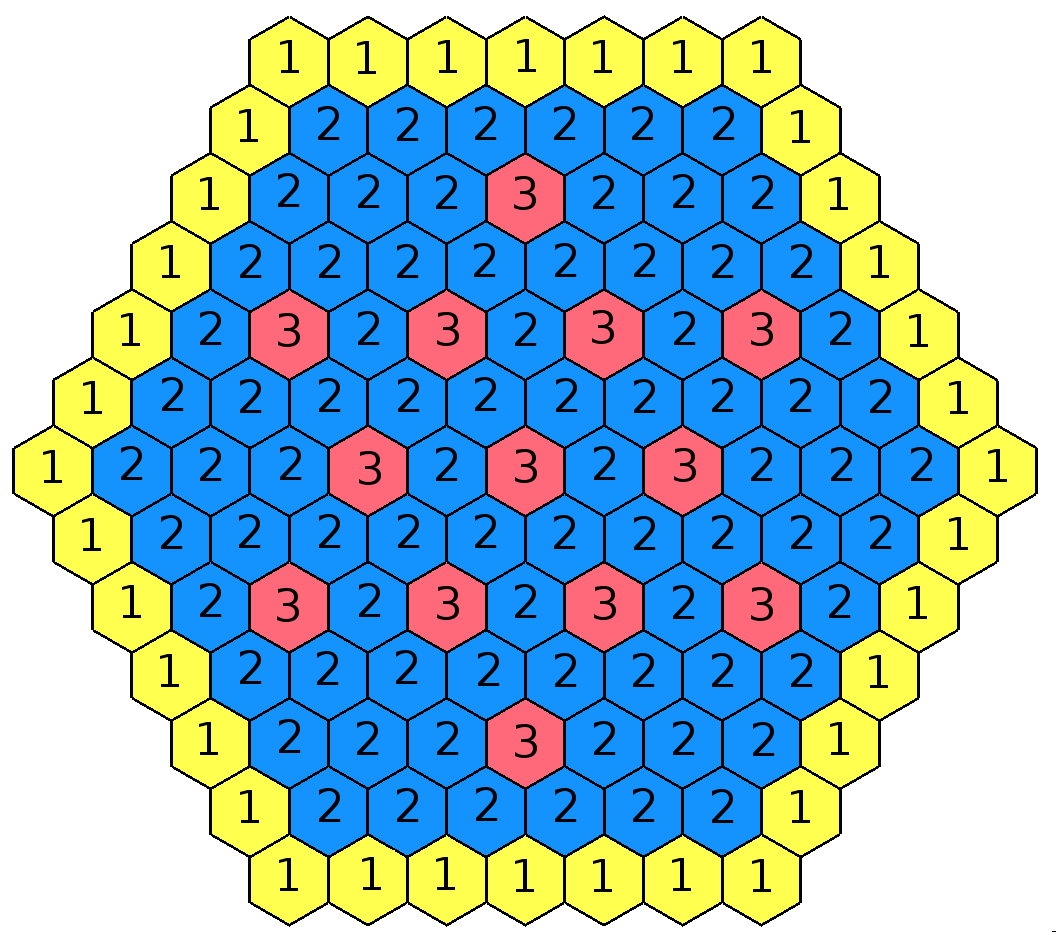
\includegraphics[width=1\linewidth]{ts_iaea/1.png}
		\column{0.5\textwidth}
			\begin{itemize}
				\item Without reflector
				\vspace{2mm}
%				\visible<2,3>{
				\item One group of \textit{instantaneous} and \textit{delayed} neutrons
				%}
				\vspace{2mm}
%				\visible<3>{
				\item Modeling effect of \textit{immersion} or \textit{extraction} of control rods
				%}
			\end{itemize}
	\end{columns}
\end{frame}

\begin{frame}{Scenario}
Define the scenario of process:
\vspace{2mm}
\begin{enumerate}
\item The spectral problem is solved (initial condition);
\vspace{2mm}

\item Calculation for the non-stationary model in the range 0 to 0.5 sec;
\vspace{2mm}

\item At a moment of 0.1 sec the value $\Sigma_a$ for the zone 3 changes to $\pm$ 0.000625.

\end{enumerate}
\end{frame}

\subsection{Software}
\begin{frame}{Software}
\begin{center}
	{
\includegraphics[width=0.4\linewidth] {gmsh.png}}
    \hfill
    
\includegraphics[width=0.49\linewidth] {slepc.png}
    \vfill
	
\includegraphics[width=0.49\linewidth] {fenics.png}
    \hfill
	
\includegraphics[width=0.49\linewidth] {python.png}
\end{center}
\end{frame}

\subsection{Computational results}
\begin{frame}{Nuclear power}
\begin{center}
    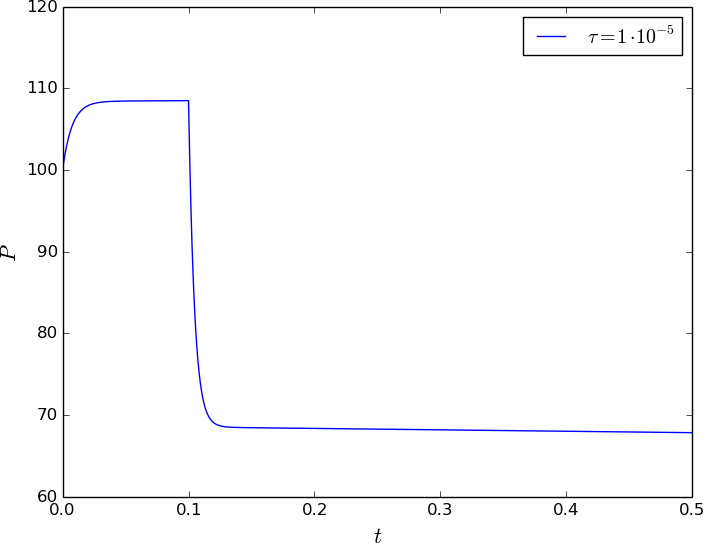
\includegraphics[width=0.49\linewidth] {ts_iaea/power_down.png}
    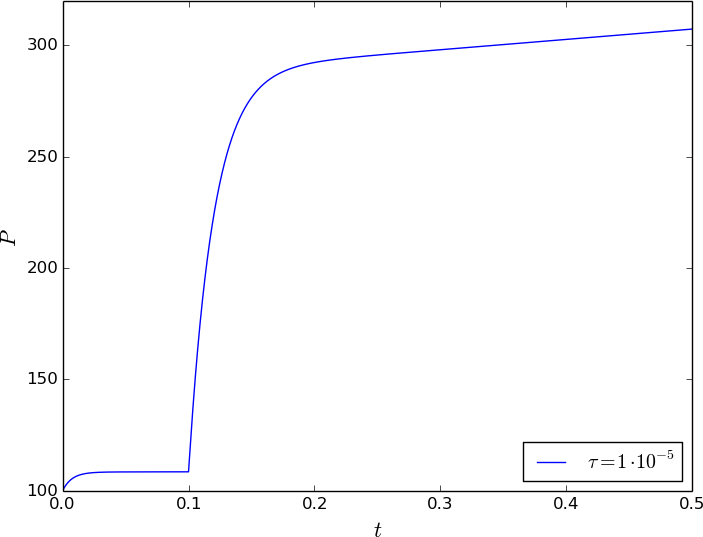
\includegraphics[width=0.49\linewidth] {ts_iaea/power_up.png}
    \\
	Nuclear power for immersion (left) and extraction (right).
    \[
    P(t)=a \sum_{g=1}^G\int_{\Omega}\Sigma_{fg}\phi_g d\bm x,
    \]
    where $a$ -- normalization factor.
\end{center}
\end{frame}

\begin{frame}{Error}
\begin{center}
    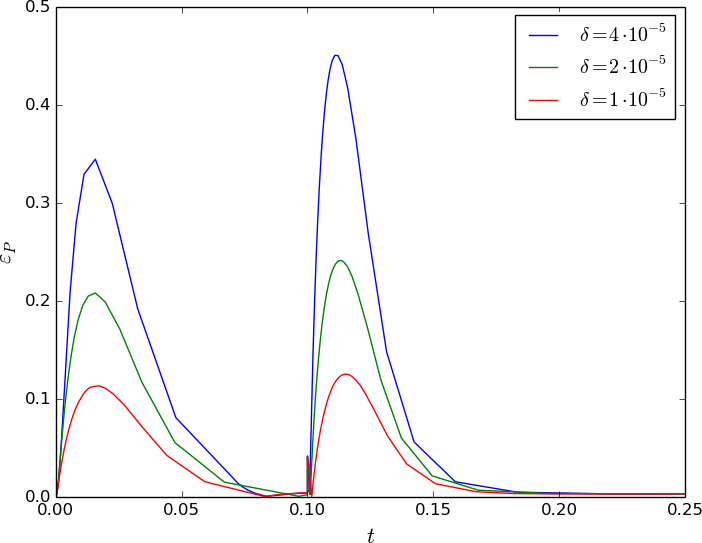
\includegraphics[width=0.49\linewidth] {ts_iaea/delta_down.png}
    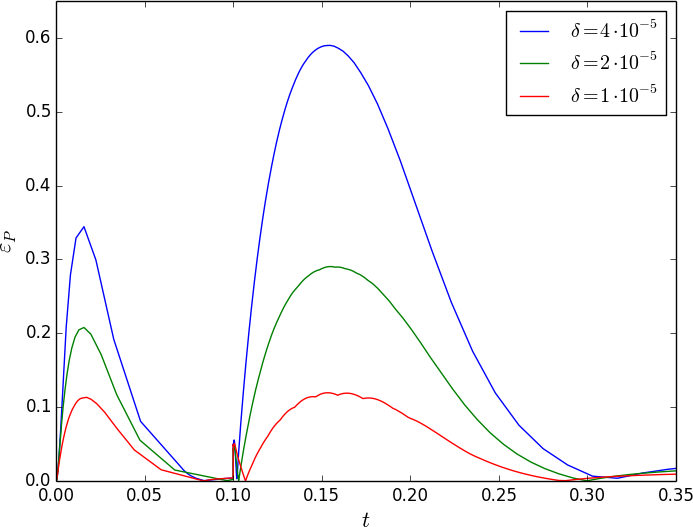
\includegraphics[width=0.49\linewidth] {ts_iaea/delta_up.png}
    \\
	Error for immersion (left) and extraction (right).
     \[
     \epsilon_P(t) = | P_{ref} - P|,
     \]
     where $P_{ref}$ -- reference solution.
\end{center}
\end{frame}


\begin{frame}{Time step}
\begin{center}
	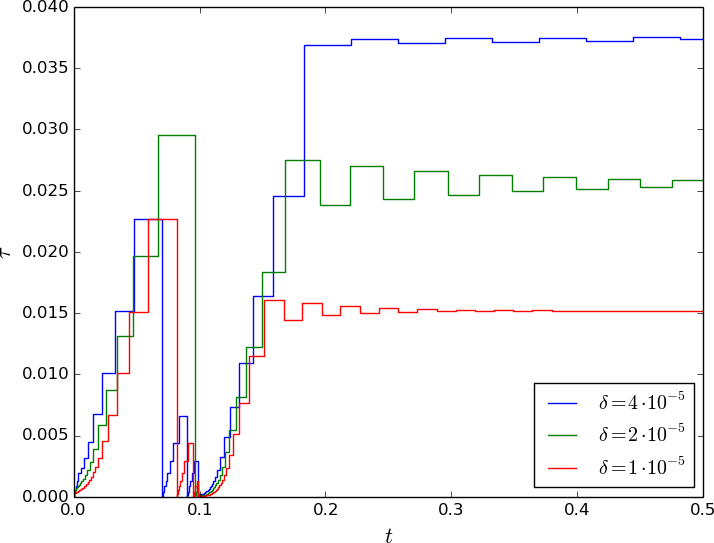
\includegraphics[width=0.49\linewidth] {ts_iaea/step_down.png}
    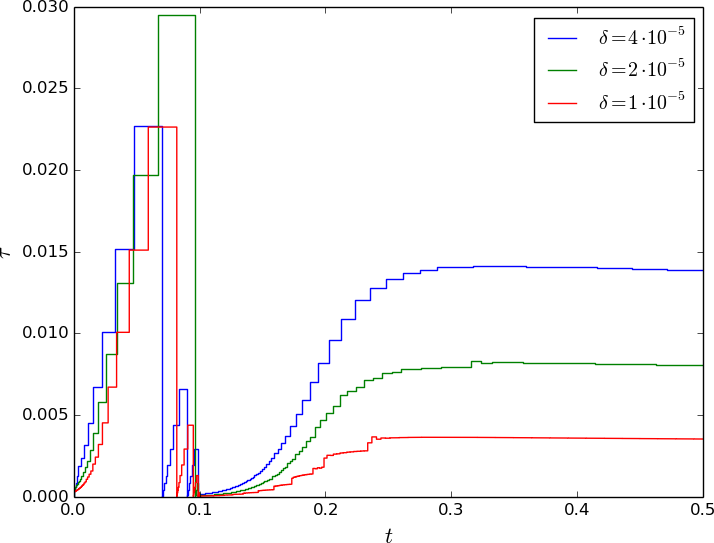
\includegraphics[width=0.49\linewidth] {ts_iaea/step_up.png}
    \\
	Time steps for immersion (left) and extraction (right).
\end{center}
\end{frame}

\begin{frame}{Counting time and number of steps}
\begin{table}[htp]
\begin{center}
\begin{tabular}{ccrrcrr}
&\multicolumn{3}{c}{immersion} & \multicolumn{3}{c}{extraction}\\
\hline
$\delta$ & max($\epsilon_P$) & $n$ & $t$, sec & max($\epsilon_P$)  & $n$ & $t$, sec \\
\hline
$4\cdot 10^{-5}$ & 0.450 & 136 & 16 & 0.590 & 241 & 35 \\
$2\cdot 10^{-5}$ & 0.241 & 159 & 20 & 0.290 & 373 & 62 \\
$1\cdot 10^{-5}$ & 0.125 & 270 & 37 & 0.120 & 773 & 145 \\
\hline
\end{tabular}
\end{center}
\end{table}
\vspace{5mm}

Reference solution: fixed time step $10^{-5}$, number of steps -- 50000,  counting time -- 2130 sec. 

\vfill

\end{frame}

\section*{Conclusion}
\begin{frame}{Acknowledgements}
This work was supported by the Russian Foundation for Basic Research (grants 16-08-01215 and 18-31-00315) and by the grant of the Russian Federation Government 14.Y26.31.0013.
\end{frame}


\begin{frame}{Conclusion}
\begin{itemize}
\item
An algorithm for automatic time step selection for numerical solution of neutron diffusion problems  has been developed.
\vspace{2mm}

\item
The solution is obtained using guaranteed stable implicit schemes, and the step choice is performed with the use of the solution obtained by an explicit scheme.
\vspace{2mm}

\item
Calculation results obtained for a neutron diffusion problems demonstrate reliability of the proposed algorithm for time step choice.
\end{itemize}

\vfill
\begin{center}
Thank you for your attention!
\end{center}

\end{frame}

\end{document}
